\documentclass[tikz,border=10pt]{standalone}
\usepackage{amsmath}
\usepackage{tikz}
\usetikzlibrary{arrows.meta, positioning, calc, shapes.geometric}

\begin{document}
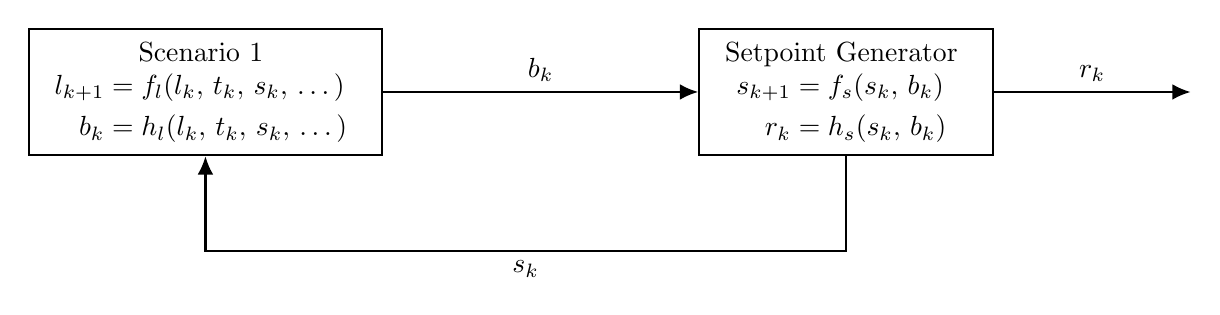
\begin{tikzpicture}[
  block/.style = {draw, thick, minimum height=3em, minimum width=6em, align=center},
  arrow/.style = {thick, -{Latex[width=2mm]}},
  node distance=2.5cm and 2.5cm
]

  % Signal Generator
  \node[block] (siggen) {
    \begin{tabular}{c}
      Setpoint Generator \\
      $\begin{aligned}
        s_{k+1} &= f_s(s_k,\,b_k) \\
        r_k &= h_s(s_k,\,b_k)
      \end{aligned}$
    \end{tabular}
  };

  % Scenario / Button block (explicit positioning)
  \node[block, left=4cm of siggen] (button) {
    \begin{tabular}{c}
      Scenario 1 \\
      $\begin{aligned}
        l_{k+1} &= f_l(l_k,\,t_k,\,s_k,\,\dots) \\
        b_k &= h_l(l_k,\,t_k,\,s_k,\,\dots)
      \end{aligned}$
    \end{tabular}
  };

  % b_k from button to signal generator
  \draw[arrow] (button.east) -- node[above] {$b_k$} (siggen.west);

  % r_k output
  \draw[arrow] (siggen.east) -- ++(2.5,0) node[midway,above] {$r_k$};

  % Feedback: s_k from siggen to button (down, left, up)
  \coordinate (sk_down) at ($(siggen.south)+(0,-1.2)$);
  \coordinate (sk_left) at ($(button.south)+(0,-1.2)$);

  \draw[arrow]
    (siggen.south)
      -- (sk_down)
      -- node[midway,below] {$s_k$} (sk_left)
      -- (button.south);

\end{tikzpicture}
\end{document}
